\documentclass[12pt]{article}
\usepackage[margin=1in]{geometry}
\usepackage{amsmath, amssymb, amsthm, graphicx, hyperref}
\usepackage{amsmath}
\usepackage{enumerate}
\usepackage{fancyhdr}
\usepackage{multirow, multicol}
\usepackage{tikz}
\usepackage{wrapfig}
\pagestyle{fancy}
\usepackage{titlesec}
\usepackage{lastpage}
\usepackage{multirow}
\usepackage{indentfirst}
\fancyhead[LO]{JACK Z}
\fancyhead[RO]{Page \thepage\ of \pageref{LastPage}}
\usepackage{comment}
\newtheorem{definition}{Definition}
\usepackage{amsmath}
\usepackage{booktabs}
\usepackage{xcolor}
\usepackage{tcolorbox}  % For creating styled boxes
\tcbuselibrary{most}
\usepackage{tcolorbox} % for creating colored or framed text boxes
\tcbuselibrary{breakable} % allows tcolorboxes to break across pages

\definecolor{examplebg}{RGB}{255, 228, 225} % Light red background
\tcbuselibrary{theorems} 
\usepackage{graphicx}
\usepackage{booktabs} % For better table formatting
\usepackage{caption} % Essential for \captionof
\usepackage{tcolorbox} % For creating colored boxes
\tcbuselibrary{most} % Load most libraries for tcolorbox

\newtcbtheorem[number within=subsection]{Note}{Note}{
    colback=Black!5,
    colframe=white!35!black,
    fonttitle=\bfseries,
    colbacktitle=blue!85!black,
    coltitle=white,
    enhanced,
    attach boxed title to top left={yshift=-2mm, xshift=2mm},
    boxed title style={sharp corners},
    sharp corners
}{Not}

\newtcbtheorem[number within=subsection]{Definition}{Definition}{
    colback=blue!5,
    colframe=blue!35!black,
    fonttitle=\bfseries,
    colbacktitle=blue!85!black,
    coltitle=white,
    enhanced,
    attach boxed title to top left={yshift=-2mm, xshift=2mm},
    boxed title style={sharp corners},
    sharp corners
}{def}

\newtcbtheorem[number within=subsection]{mytheorem}{Theorem}{
    colback=orange!5,      % Background color of the box
    colframe=orange,     % Border color of the box
    coltitle=white,     % Color of theorem title
    colbacktitle=orange!85!black,, % Background color for the title
    fonttitle=\bfseries,
    title after break={Theorem \csname the\tcbcounter\endcsname\ -- Continued}, % for continued theorems
    enhanced,
    attach boxed title to top left={yshift=-2mm, xshift=2mm},
    boxed title style={sharp corners, colframe=black},
    sharp corners,
    separator sign none % no sign between title and theorem text
}{thm}


\usepackage{lipsum} % 生成示例文本
\usepackage{fancyhdr}

\pagestyle{fancy}
\fancyfoot[C]{%
  \begin{tcolorbox}[colback=blue!10, colframe=blue!35, boxrule=0.5pt, 
  sharp corners=south, boxsep=2pt, width=0.25\textwidth, 
  arc=3mm, enhanced, shadow=drop shadow]
    \centering
    {\textbf{\textcopyright\ \textit{Novel Prep}}}
  \end{tcolorbox}
}

% Define custom colors
\definecolor{deepblue}{rgb}{0.0, 0.18, 0.39}
\definecolor{deepred}{rgb}{0.6, 0, 0}

% Define theorem style
\newtheoremstyle{beautifulthm}
  {10pt} % Space above
  {10pt} % Space below
  {\itshape} % Body font
  {} % Indent amount
  {\bfseries\color{deepblue}} % Theorem head font
  {.} % Punctuation after theorem head
  {.5em} % Space after theorem head
  {} % Theorem head spec

\theoremstyle{beautifulthm}
\newtheorem{theorem}{Theorem}[section]

\begin{document}

\title{AP Calculus AB\&BC}
\author{Hongjun Zeng}
\maketitle
\lipsum[1-10] 

\tableofcontents
\begin{document}
\section{Limits and Continuity}
\section{Differentiation: Definition and Fundamental Properties}
\section{Differentiation: Composite, Implicit, and Inverse Function}
\section{Application of Differentiation}
\section{Analytical Applications of Differentiation}
\section{Accumulations of Change}
\section{Differential Equations}
\section{Applications of Integration}
\newpage

\subsection{Average
Value of a Function on an
Interval}

\subsubsection{The Mean Value Theorem for Integrals}

\begin{mytheorem}{Mean Value Theorem for Integrals}{}
    If $f$ is continuous on the closed interval $[a, b]$, then there exists a number $c$ in the closed interval $[a, b]$ such that
\[
\int_a^b f(x) \, dx = f(c)(b - a).
\]


\begin{minipage}{\linewidth}
    \centering
    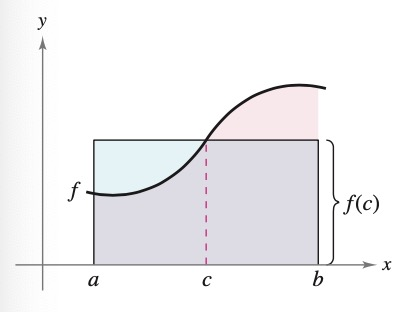
\includegraphics[width=0.30\linewidth]{Example_63.jpg} 
\end{minipage}
\end{mytheorem}


\textbf{Proof:}

\textbf{Case 1:} If $f$ is constant on the interval $[a, b]$, then the theorem is clearly valid because $c$ can be any point in $[a, b]$.

\textbf{Case 2:} If $f$ is not constant on $[a, b]$, then, by the Extreme Value Theorem, you can choose $f(m)$ and $f(M)$ to be the minimum and maximum values of $f$ on $[a, b]$. Because
\[
f(m) \leq f(x) \leq f(M)
\]
for all $x$ in $[a, b]$, you can apply Theorem 4.8 to write the following:
\[
\int_a^b f(m) \, dx \leq \int_a^b f(x) \, dx \leq \int_a^b f(M) \, dx
\]
\hspace*{1cm}

\[
f(m)(b - a) \leq \int_a^b f(x) \, dx \leq f(M)(b - a)
\]
\hspace*{1cm} \textit{Apply Fundamental Theorem.}

\[
f(m) \leq \frac{1}{b - a} \int_a^b f(x) \, dx \leq f(M)
\]
\hspace*{1cm} \textit{Divide by $b - a$.}

From the third inequality, you can apply the Intermediate Value Theorem to conclude that there exists some $c$ in $[a, b]$ such that
\[
f(c) = \frac{1}{b - a} \int_a^b f(x) \, dx \quad \text{or} \quad f(c)(b - a) = \int_a^b f(x) \, dx.
\]


\subsubsection{Average Value of a Function}
The value of $f(c)$ given in the Mean Value Theorem for Integrals is called the \textbf{average value} of $f$ on the interval $[a, b]$.

\begin{mytheorem}{Average Value of a Function on an Interval}{}
    If $f$ is integrable on the closed interval $[a, b]$, then the \textbf{average value} of $f$ on the interval is
\[
\frac{1}{b - a} \int_a^b f(x) \, dx.
\]
\end{mytheorem}

\begin{tcolorbox}[colback=examplebg, colframe=red!75!black, title=\textbf{EXAMPLE 1: Finding the Average Value of a Function}, fonttitle=\bfseries, sharp corners]
Find the average value of $f(x) = 3x^2 - 2x$ on the interval $[1, 4]$.


\tcblower
\textbf{Solution:} 
 The average value is
\[
\frac{1}{b - a} \int_a^b f(x) \, dx = \frac{1}{4 - 1} \int_1^4 \big(3x^2 - 2x\big) \, dx
\]
\[
= \frac{1}{3} \left[ x^3 - x^2 \right]_1^4
\]
\[
= \frac{1}{3} \big[ 64 - 16 - (1 - 1) \big]=16
\]

\end{tcolorbox}

\begin{tcolorbox}[colback=examplebg, colframe=red!75!black, title=\textbf{EXAMPLE 2: Average Velocity}, fonttitle=\bfseries, sharp corners]
Show that the \textbf{average velocity} of a car over a time interval $[t_1, t_2]$ is the same as the \textbf{average} of its velocities during the trip.



\tcblower
\textbf{Solution:} 
If $s(t)$ is the displacement of the car at time $t$, then, by definition, the \textbf{average velocity} of the car over the interval is
\[
\frac{\Delta s}{\Delta t} = \frac{s(t_2) - s(t_1)}{t_2 - t_1}.
\]

On the other hand, the \textbf{average value} of the velocity function on the interval is
\[
v_{\text{avg}} = \frac{1}{t_2 - t_1} \int_{t_1}^{t_2} v(t) \, dt = \frac{1}{t_2 - t_1} \int_{t_1}^{t_2} s'(t) \, dt
\]
\[
= \frac{1}{t_2 - t_1} \big[s(t_2) - s(t_1)\big] \quad \text{(by the Net Change Theorem)}
\]
\[
= \frac{s(t_2) - s(t_1)}{t_2 - t_1} = \text{average velocity}.
\]
\end{tcolorbox}


\subsection{Position,
Velocity, and Acceleration}


\subsubsection{Integrating Velocity to Find Position}

\begin{mytheorem}{Integral of Velocity}{}
    The \textbf{fundamental theorem of calculus} states that the integral of velocity over a specific time interval gives the change in position during that interval. The position function $s(t)$ is given by:
\[
s(t) = \int v(t) \, dt + C,
\]
where $C$ represents the constant of integration, corresponding to the initial position.
\end{mytheorem}

\begin{mytheorem}{Displacement}{}
    The change in position, also called the \textbf{displacement}, is defined as the difference between the final position $s_f$ and the initial position $s_i$:
\[
\text{displacement} = s_f - s_i = \Delta s = \int v(t) \, dt.
\]
\end{mytheorem}



\begin{mytheorem}{distance traveled}{}
The \textbf{distance traveled} measures the total length of the path taken by the object, regardless of direction. It is given by:
\[
\text{distance traveled} = \int |v(t)| \, dt,
\]
where the absolute value of the velocity is integrated to account for changes in direction.
\end{mytheorem}

\begin{tcolorbox}[colback=examplebg, colframe=red!75!black, title=\textbf{EXAMPLE 1: Position }, fonttitle=\bfseries, sharp corners]
Suppose an object has a velocity function $v(t) = 2t + 5$ with an initial position $s(0) = 10$. Find the position function $s(t)$.


\tcblower
\textbf{Solution:} 
 To find the position function $s(t)$, we integrate the velocity function with respect to time. Mathematically, this is represented as:
\[
s(t) = \int (2t + 5) \, dt + 10
\]

Integrating this function and adding the initial position, we get:
\[
s(t) = \frac{1}{2}t^2 + 5t + 10.
\]
\end{tcolorbox}



\begin{tcolorbox}[colback=examplebg, colframe=red!75!black, title=\textbf{EXAMPLE 2: Displacement \& Distance}, fonttitle=\bfseries, sharp corners]

Given an object's velocity function $v(t) = 3t - 2$ on the interval $[1, 4]$ with an initial position of $s(1) = 5$, find the displacement and distance traveled.

\tcblower
\textbf{Solution:} 
The displacement is the change in position from $t = 1$ to $t = 4$. Mathematically, it's represented as:
\[
\text{displacement} = s(4) - s(1) = \int_{1}^{4} (3t - 2) \, dt.
\]

Let's integrate the velocity function over the given interval:
\[
\text{displacement} = \left[ \frac{3}{2}t^2 - 2t \right]_1^4.
\]

The distance traveled is:
\[
\text{distance traveled} = \int_{1}^{4} |3t - 2| \, dt.
\]

Since the velocity function is always positive over the given interval, we can remove the absolute value symbols and integrate normally:
\[
\text{distance traveled} = \int_{1}^{4} (3t - 2) \, dt = \left[ \frac{3}{2}t^2 - 2t \right]_1^4.
\]

Evaluating this integral using the fundamental theorem of calculus yields:
\[
\text{displacement} = \text{distance traveled} = \frac{9}{2}.
\]
\end{tcolorbox}




\newpage
\subsubsection{Integrating Acceleration to Find Velocity
}

\begin{mytheorem}{Integrating Acceleration to Find Velocity}
     to find an object's velocity at any time, we integrate its acceleration function. The integral of acceleration with respect to time yields the change in velocity over a given interval:
\[
v(t) = \int a(t) \, dt + C.
\]

In this equation, $C$ represents the constant of integration, which corresponds to the initial velocity. Just like finding the final position, we need to add the initial velocity to the result of our integral in order to find the final velocity.
\end{mytheorem}

\begin{tcolorbox}[colback=examplebg, colframe=red!75!black, title=\textbf{EXAMPLE 3: Find the Integral of the Function}, fonttitle=\bfseries, sharp corners]
A particle moves along the $y$-axis with an acceleration of $a(t) = 2$, where $t$ is time in seconds. The particle's velocity at $t = 2$ is 5 cm/sec. The position of the particle at $t = 2$ is 10 cm. What is the position of the particle at $t = 6$?


\tcblower
\textbf{Solution:} 
First, find the velocity:
\[
v(t) = \int a(t) \, dt = \int 2 \, dt = 2t + C.
\]

Using $v(2) = 5$:
\[
5 = 4 + C \quad \Rightarrow \quad C = 1.
\]

Thus, $v(t) = 2t + 1$.

Now, find the position:
\[
x(t) = \int v(t) \, dt = \int (2t + 1) \, dt = t^2 + t + C.
\]

Using $x(2) = 10$:
\[
10 = 4 + 2 + C \quad \Rightarrow \quad C = 4.
\]

Thus, $x(t) = t^2 + t + 4$.

At $t = 6$:
\[
x(6) = 6^2 + 6 + 4 = 36 + 6 + 4 = 46 \, \text{cm}.
\]
\end{tcolorbox}




\subsection{ Using Accumulation Functions and Definite Integrals}


\begin{Definition}{Accumulation Functions }{}
    The integral represents the accumulation of a quantity over a given interval. Mathematically, it is defined as:

\[
\int_a^b f(x) \, dx
\]

where:
\begin{itemize}
    \item $f(x)$ is the function representing the rate of change or density of the quantity being accumulated.
    \item $a$ and $b$ are the bounds of the interval over which accumulation occurs.
\end{itemize}

The integral computes the total accumulation of $f(x)$ from $x = a$ to $x = b$, effectively summing the infinitely small contributions $f(x) \, dx$ over the interval $[a, b]$.
\end{Definition}
\begin{minipage}{\linewidth}
    \centering
    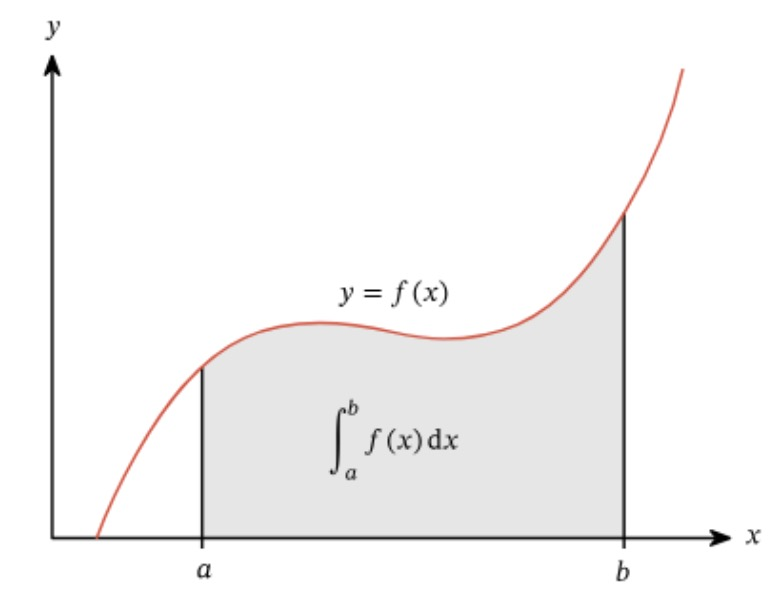
\includegraphics[width=0.60\linewidth]{Example_64.jpg} 
\end{minipage}




\begin{Note}{Accumulation Function: Steps to Follow}{}

\begin{enumerate}
    \item Identify the rate of change function.
    \item Set up the definite integral to find the net change.
    \item Evaluate the integral.
    \item Use any provided initial condition to complete the problem.
\end{enumerate}
    
\end{Note}


\vspace{1cm}

\begin{tcolorbox}[colback=examplebg, colframe=red!75!black, title=\textbf{EXAMPLE 1: Find the Integral of the Function}, fonttitle=\bfseries, sharp corners]

Rate of consumption of oil in the United States during the 1980s (in billions of barrels per year) is modeled by the function:
\[
R(t) = 27.08 e^{\frac{t}{25}}
\]
where $t$ is the number of years after January 1, 1980. Find the total consumption of oil in the United States during the 1980s.

\tcblower
\textbf{Solution:}

The total consumption of oil is given by the integral:
\[
\int_{0}^{10} R(t) \, dt = 332.965 \, \text{billion barrels}
\]

\end{tcolorbox}



\vspace{1cm}

\begin{tcolorbox}[colback=examplebg, colframe=red!75!black, title=\textbf{EXAMPLE 2: Find the Integral of the Function}, fonttitle=\bfseries, sharp corners]

The population of a city is modeled by the function:
\[
P(t) = 5000 e^{0.03t}
\]
where $t$ is the number of years since the year 2000. Find the total population growth between the years 2000 and 2020.

\tcblower
\textbf{Solution:}

To find the total population growth over the 20-year period, we compute the definite integral:
\[
\int_{0}^{20} P(t) \, dt = \int_{0}^{20} 5000 e^{0.03t} \, dt
\]

Evaluating the integral:
\[
= \left[ \frac{5000}{0.03} e^{0.03t} \right]_{0}^{20}
= \frac{5000}{0.03} \left( e^{0.6} - 1 \right)
\]
\[
= 166,666.67 \left(1.8221 - 1 \right)
= 136,800 \, \text{people}
\]

\end{tcolorbox}





\newpage 


\newpage
\begin{tcolorbox}[colback=examplebg, colframe=red!75!black, title=\textbf{EXAMPLE 4:}, fonttitle=\bfseries, sharp corners]
For $0 \leq t \leq 31$, the rate of change of the number of mosquitoes on Tropical Island at time $t$ days is modeled by 
\[
R(t) = 5\sqrt{t} \cos\left(\frac{t}{5}\right) \quad \text{mosquitoes per day}.
\]
There are 1000 mosquitoes on Tropical Island at time $t = 0$.

\begin{enumerate}
    \item[(a)] Show that the number of mosquitoes is increasing at time $t = 6$.
    \item[(b)] At time $t = 6$, is the number of mosquitoes increasing at an increasing rate, or is the number of mosquitoes increasing at a decreasing rate? Give a reason for your answer.
    \item[(c)] According to the model, how many mosquitoes will be on the island at time $t = 31$? Round your answer to the nearest whole number.
\end{enumerate}


\tcblower
\textbf{Solution:} 

\begin{enumerate}
    \item[(a)] To determine whether the number of mosquitoes is increasing at time $t = 6$, we evaluate $R(6)$. Since $R(t)$ represents the rate of change of the number of mosquitoes, if $R(6) > 0$, the number of mosquitoes is increasing.

    \[
    R(6) = 5\sqrt{6} \cos\left(\frac{6}{5}\right).
    \]

    Calculating $\cos\left(\frac{6}{5}\right)$, we find that $R(6) > 0$. Thus, the number of mosquitoes is increasing at $t = 6$.

    \item[(b)] To determine if the number of mosquitoes is increasing at an increasing or decreasing rate at $t = 6$, we evaluate the derivative of $R(t)$, denoted as $R'(t)$. 
    \[
    R'(t) = 5 \frac{1}{2\sqrt{t}} \cos\left(\frac{t}{5}\right) - 5\sqrt{t} \sin\left(\frac{t}{5}\right) \cdot \frac{1}{5}.
    \]

    At $t = 6$, we substitute and calculate $R'(6)$. Based on calculations, $R'(6) < 0$, so the number of mosquitoes is increasing at a decreasing rate.

    \item[(c)] To find the number of mosquitoes at $t = 31$, we integrate $R(t)$ over the interval $[0, 31]$ and add the initial population of 1000 mosquitoes.

    \[
    \text{Number of mosquitoes} = 1000 + \int_0^{31} 5\sqrt{t} \cos\left(\frac{t}{5}\right) \, dt.
    \]

    Using numerical methods or a calculator, the integral evaluates to approximately $139.51$. Adding this to the initial population:
    \[
    \text{Number of mosquitoes} \approx 1000 + 139 = 1139.
    \]
\end{enumerate}
\end{tcolorbox}

\newpage

\subsection{Finding the Area Between
Curves (Expressed as
Functions of x)}
\begin{mytheorem}{Area of a Region Between Two Curves (X-Axis)}{}
    If $f$ and $g$ are continuous on $[a, b]$ and $g(x) \leq f(x)$ for all $x$ in $[a, b]$, then the area of the region bounded by the graphs of $f$ and $g$ and the vertical lines $x = a$ and $x = b$ is

\[
A = \int_a^b \big[f(x) - g(x)\big] \, dx.
\]
\end{mytheorem}
\begin{minipage}{\linewidth}
    \centering
    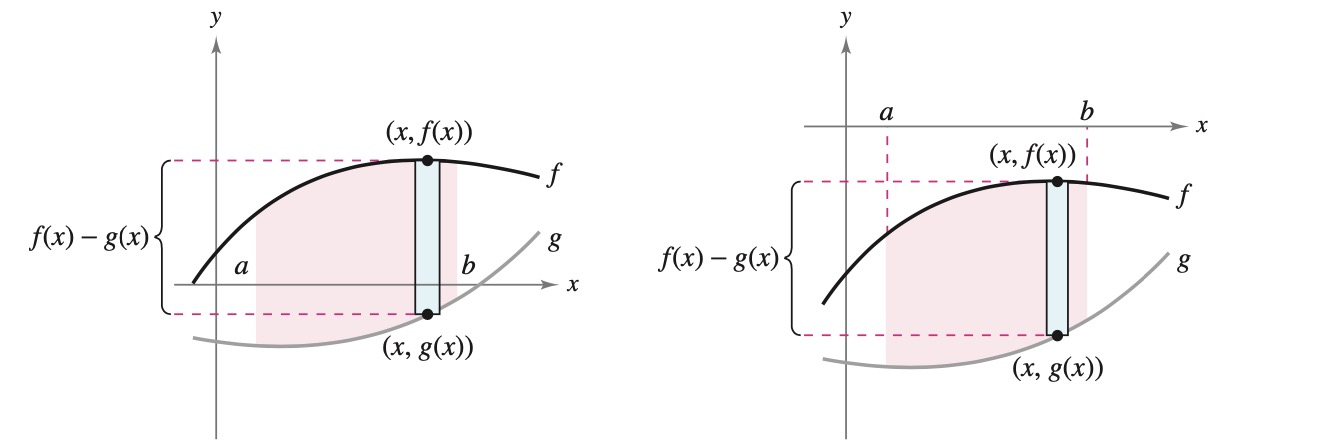
\includegraphics[width=0.90\linewidth]{Example_65.jpg} 
\end{minipage}


\begin{tcolorbox}[colback=examplebg, colframe=red!75!black, title=\textbf{EXAMPLE 1: Finding the Area of a Region Between Two Curves}, fonttitle=\bfseries, sharp corners]

Find the area of the region bounded by the graphs of $y = x^2 + 2$, $y = -x$, $x = 0$, and $x = 1$.

\tcblower
\textbf{Solution:} 
Let $g(x) = -x$ and $f(x) = x^2 + 2$. Then $g(x) \leq f(x)$ for all $x$ in $[0, 1]$. So, the area of the representative rectangle is
\[
\Delta A = [f(x) - g(x)] \Delta x = [(x^2 + 2) - (-x)] \Delta x.
\]

And the area of the region is
\[
A = \int_a^b \big[f(x) - g(x)\big] \, dx
\]
\[
= \int_0^1 \big[(x^2 + 2) - (-x)\big] \, dx
\]
\[
= \int_0^1 \big(x^2 + 2 + x\big) \, dx.
\]

Now, integrate term by term:
\[
A = \left[\frac{x^3}{3} + \frac{x^2}{2} + 2x\right]_0^1 =  \frac{17}{6}.
\]
\end{tcolorbox}


\begin{tcolorbox}[colback=examplebg, colframe=red!75!black, title=\textbf{EXAMPLE 2: A Region Lying Between Two Intersecting Graphs}, fonttitle=\bfseries, sharp corners]

\textbf{Find the area of the region bounded by the graphs of} 
\[
f(x) = e^x \quad \text{and} \quad g(x) = x + 2.
\]

\tcblower
\textbf{Solution:} 

To find the $x$-coordinates of the points of intersection, set $f(x)$ and $g(x)$ equal to each other and solve for $x$:
\[
e^x = x + 2
\]
This equation cannot be solved algebraically, but numerical methods give approximate solutions:
\[
x \approx 0 \quad \text{and} \quad x \approx 1.
\]

So, $a = 0$ and $b = 1$. Because $g(x) \leq f(x)$ for all $x$ in the interval $[0, 1]$, the area of the region is:
\[
A = \int_{0}^{1} [e^x - (x + 2)] \, dx
\]

Evaluating the integral:
\[
A = \left[ e^x - \frac{x^2}{2} - 2x \right]_0^1
\]
\[
= \left( e - \frac{1}{2} - 2 \right) - \left( 1 - 0 - 0 \right)
\]
\[
= (e - 2.5) - 1
\]
\[
= e - 3.5
\]


\[
\boxed{A = e - 3.5}
\]


\end{tcolorbox}





\begin{tcolorbox}[colback=examplebg, colframe=red!75!black, title=\textbf{EXAMPLE 3: Finding the Area of a Region Between Two Curves}, fonttitle=\bfseries, sharp corners]
\begin{minipage}{\linewidth}
    \centering
    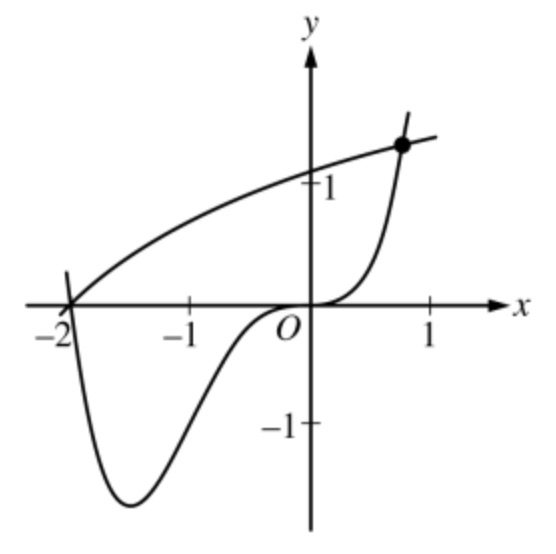
\includegraphics[width=0.40\linewidth]{Example_66.jpg} 
\end{minipage}

Graph depicts the functions $f(x)$ and $g(x)$ defined below.

Let $f$ and $g$ be the functions defined by $f(x) = \ln(x + 3)$ and $g(x) = x^4 + 2x^3$. The graphs of $f$ and $g$, shown in the figure above, intersect at $x = -2$ and $x = B$, where $B > 0$.

Find the area of the region enclosed by the graphs of $f$ and $g$.
\tcblower
\textbf{Solution:} 
To find the area of the region enclosed by the graphs of $f(x) = \ln(x + 3)$ and $g(x) = x^4 + 2x^3$, we calculate the definite integral of the difference between the two functions over the interval $[-2, B]$ (where $B$ is the intersection point such that $B > 0$).

The enclosed area is given by:
\[
A = \int_{-2}^B \big[f(x) - g(x)\big] \, dx.
\]

Substitute the given functions:
\[
A = \int_{-2}^B \big[\ln(x + 3) - (x^4 + 2x^3)\big] \, dx.
\]

\textbf{Step 1: Determine $B$.} To find the value of $B$, solve the equation $f(x) = g(x)$:
\[
\ln(x + 3) = x^4 + 2x^3.
\]
This must be solved numerically or graphically to find the exact value of $B$.

\textbf{Step 2: Compute the integral.} 
we can find that the value of $B$ is $0.781975$. Now, rewrite and evaluate our definite integral to find the area:

\[
A = \int_{-2}^{0.781} \big[\ln(x + 3) - (x^4 + 2x^3)\big] \, dx = 3.604.
\]
\end{tcolorbox}

\newpage
\subsection{ Finding the Area Between
Curves (Expressed as
Functions of y)}

\begin{mytheorem}{Area of a Region Between Two Curves(Y-Axis)}{}

To find the area between two curves $y = f(x)$ and $y = g(x)$ over an interval $[c, d]$, we'll be integrating with respect to $y$.

The formula for the area is given by, where $f(y) > g(y)$:
\[
A = \int_c^d \big| f(y) - g(y) \big| \, dy.
\]

Here, $[c, d]$ is the interval on the $y$-axis where the curves intersect. We take the absolute value to ensure we're dealing with positive areas.
\end{mytheorem}

\begin{minipage}{\linewidth}
    \centering
    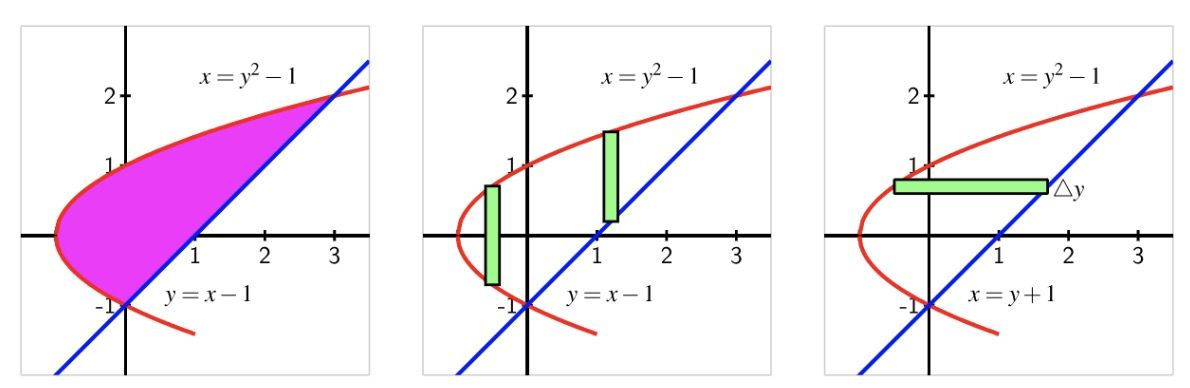
\includegraphics[width=1\linewidth]{Example_67.jpg} 
\end{minipage}




\begin{Note}{Common Pitfalls}{}
    \begin{itemize}
    \item \textbf{Wrong Order of Functions:} Using $g(y) - f(y)$ instead of $f(y) - g(y)$ can lead to negative areas.
    \item \textbf{Incorrect Bounds:} Misidentifying the points of intersection or using incorrect limits can lead to errors.
    \item \textbf{Curve Crossing:} If $f(y)$ and $g(y)$ cross within $[c, d]$, the integral must be split at the crossing point to avoid incorrect results.
\end{itemize}
\end{Note}

\begin{tcolorbox}[colback=examplebg, colframe=red!75!black, title=\textbf{EXAMPLE 1: Horizontal Representative Rectangles}, fonttitle=\bfseries, sharp corners]
Find the area of the region bounded by the graphs of $x = 3 - y^2$ and $x = y + 1$.


\tcblower
\textbf{Solution:} 
Consider
\[
g(y) = 3 - y^2 \quad \text{and} \quad f(y) = y + 1.
\]

These two curves intersect when $y = -2$ and $y = 1$, as shown in Figure 7.9. Because $f(y) \leq g(y)$ on this interval, you have
\[
\Delta A = \big[g(y) - f(y)\big] \Delta y = \big[(3 - y^2) - (y + 1)\big] \Delta y.
\]

So, the area is
\[
A = \int_{-2}^1 \big[(3 - y^2) - (y + 1)\big] \, dy
\]
\[
= \int_{-2}^1 \big[-y^2 - y + 2\big] \, dy.
\]

Now, integrate term by term:
\[
A = \left[-\frac{y^3}{3} - \frac{y^2}{2} + 2y\right]_{-2}^1.
\]

Substitute the bounds:
\[
A = \left(-\frac{1^3}{3} - \frac{1^2}{2} + 2(1)\right) - \left(-\frac{(-2)^3}{3} - \frac{(-2)^2}{2} + 2(-2)\right).
\]

Simplify:
\[
A = \left(-\frac{1}{3} - \frac{1}{2} + 2\right) - \left(-\frac{-8}{3} - \frac{4}{2} - 4\right)
\]
\[
= \left(-\frac{1}{3} - \frac{1}{2} + 2\right) - \left(\frac{8}{3} - 2 - 4\right).
\]

Combine terms:
\[
A = \frac{9}{2}.
\]

Thus, the area of the region is:
\[
A = \frac{9}{2}.
\]
\end{tcolorbox}

\newpage

\begin{tcolorbox}[colback=examplebg, colframe=red!75!black, title=\textbf{EXAMPLE 2: Finding the Area Between Curves ($y$ Axis)}, fonttitle=\bfseries, sharp corners]
Find the area of the region bounded by the graphs of $x = y^2$ and $x = 4$.

\tcblower
\textbf{Solution:} 

Consider the curves:
\[
f(y) = 4 \quad \text{and} \quad g(y) = y^2.
\]

These two curves intersect when $y = -2$ and $y = 2$, since $y^2 = 4$ implies $y = \pm 2$. 

The area of the region can be found using the formula:
\[
A = \int_{-2}^{2} \big[f(y) - g(y)\big] \, dy.
\]

Substitute the functions:
\[
A = \int_{-2}^{2} \big[4 - y^2\big] \, dy.
\]

Now, integrate term by term:
\[
A = \left[4y - \frac{y^3}{3}\right]_{-2}^{2}.
\]

Substitute the bounds:
\[
A = \left(4(2) - \frac{(2)^3}{3}\right) - \left(4(-2) - \frac{(-2)^3}{3}\right).
\]

Simplify:
\[
A = \left(8 - \frac{8}{3}\right) - \left(-8 + \frac{8}{3}\right).
\]

Combine terms:
\[
A = \left(\frac{24}{3} - \frac{8}{3}\right) - \left(-\frac{24}{3} + \frac{8}{3}\right)
= \frac{16}{3} + \frac{32}{3}
= \frac{48}{3}.
\]

Thus, the area of the region is:
\[
A = 16.
\]
\end{tcolorbox}


\newpage

\subsection{ Finding the Area Between
Curves( Intersect at
More Than Two Points)}

\begin{mytheorem}{Area Between
Curves}{}
  To find the area between two curves $y = f(x)$ and $y = g(x)$ over an interval $[a, b]$, we calculate:

\[
\text{Area} = \int_a^b \big|f(x) - g(x)\big| \, dx.
\]

The absolute value ensures that any negative regions are accounted for as positive contributions to the total area.  
\end{mytheorem}

\begin{tcolorbox}[colback=examplebg, colframe=red!75!black, title=\textbf{EXAMPLE 1: Curves That Intersect at More than Two Points}, fonttitle=\bfseries, sharp corners]

Find the area of the region between the graphs of 
\[
f(x) = 3x^3 - x^2 - 10x \quad \text{and} \quad g(x) = -x^2 + 2x.
\]

\begin{minipage}{\linewidth}
    \centering
    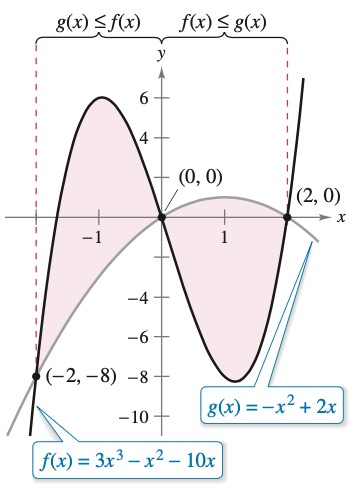
\includegraphics[width=0.30\linewidth]{Example_68.jpg} 
\end{minipage}

\tcblower
\textbf{Solution:} 
\[
3x^3 - x^2 - 10x = -x^2 + 2x,
\]

Thus, the points of intersection are $x = -2$, $x = 0$, and $x = 2$.

Notice that:
- On the interval $[-2, 0]$, $g(x) \leq f(x)$.
- On the interval $[0, 2]$, $f(x) \leq g(x)$.

So, the area can be calculated as two separate integrals:

\[
A = \int_{-2}^0 \big[(3x^3 - 12x)\big] \, dx + \int_0^2 \big[(-3x^3 + 12x)\big] \, dx = 24
\]

\end{tcolorbox}


\begin{tcolorbox}[colback=examplebg, colframe=red!75!black, title=\textbf{EXAMPLE 2: Find the Integral of the Function}, fonttitle=\bfseries, sharp corners]
The figure shows the graphs of $y = |x|$ and $y = 3 + 2x - x^2$ for $-1 \leq x \leq 3$. The $x$-coordinates of the points of intersection of the graphs are $x_1$ and $x_2$, where $x_1 < x_2$. Write a sum of integrals that represents the shaded regions. You do \textbf{NOT} need to solve for $x_1$ and $x_2$.


\begin{minipage}{\linewidth}
    \centering
    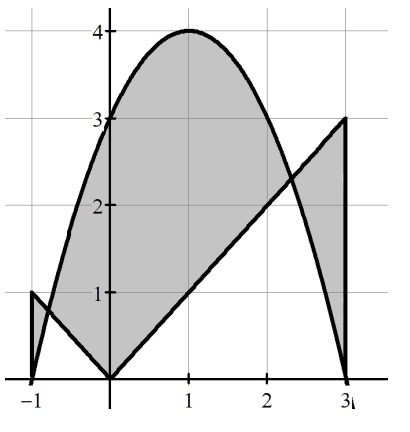
\includegraphics[width=0.40\linewidth]{Example_69.jpg} 
\end{minipage}

\tcblower
\textbf{Solution:} 
The area of the shaded region is represented by the following sum of integrals:
\[
\int_{-1}^{x_1} \big(x^2 - 3x - 3\big) \, dx 
+ \int_{x_1}^0 \big(-x^2 + 3x + 3\big) \, dx 
+ \int_0^{x_2} \big(-x^2 + x + 3\big) \, dx 
+ \int_{x_2}^3 \big(x^2 - x - 3\big) \, dx.
\]
\end{tcolorbox}


\newpage
\subsection{Volumes with Cross
Sections: Squares and
Rectangles}


So far in Previous unit, you have learned how to calculate the area between two curves. However, these curves can also be used to represent a three-dimensional object

\begin{mytheorem}{Volumes of Solids with Known Cross Sections}{}

\begin{enumerate}
    \item For cross sections of area $A(x)$ taken perpendicular to the $x$-axis:
    \[
    \text{Volume} = \int_a^b A(x) \, dx.
    \]


    \item For cross sections of area $A(y)$ taken perpendicular to the $y$-axis:
    \[
    \text{Volume} = \int_c^d A(y) \, dy.
    \]
\end{enumerate}
\end{mytheorem}

    \begin{minipage}{\linewidth}
    \centering
    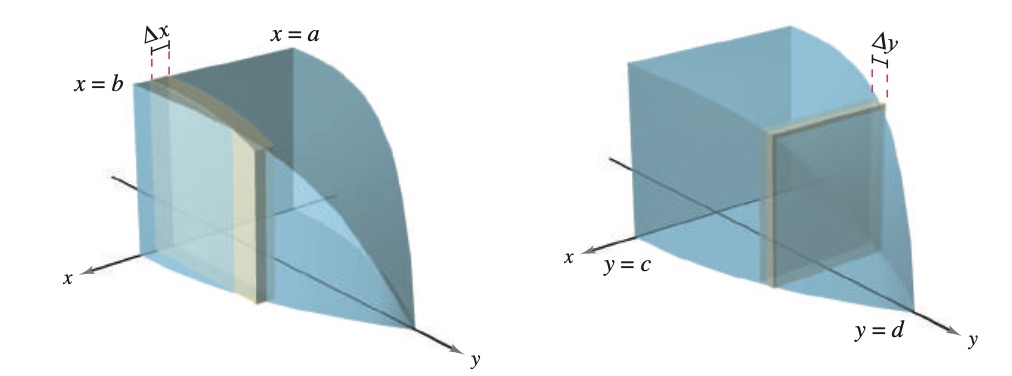
\includegraphics[width=0.9\linewidth]{Example_70.jpg} 
\end{minipage}


\newpage
\subsubsection{Rectangular Cross Sections}
\begin{mytheorem}{Rectangular Cross Sections}{}

To find the area of a rectangle, we use the formula $w \cdot h$, where $w$ is the width of the rectangle and $h$ is the height. The formula for the volume of a solid with rectangular cross sections is given by:
\[
V = \int_a^b w \cdot h \, dx.
\]

Remember, $dx$ represents the thickness!
    
\end{mytheorem}



\begin{tcolorbox}[colback=examplebg, colframe=red!75!black, title=\textbf{EXAMPLE 1: Volumes with Cross Sections: Squares and Rectangles}, fonttitle=\bfseries, sharp corners]

The base of a solid is bounded by $y = x^3$, $y = 0$, and $x = 2$. Find the volume if the cross sections, taken perpendicular to the $y$-axis, form a rectangle whose height is 6.

\tcblower
\textbf{Solution:} 

The formula for the volume of a solid with known cross sections is:
\[
V = \int_a^b w \cdot h \, dy,
\]
where $w$ is the width of the cross section, $h$ is the height, and the integral is taken with respect to $y$.

In this problem:
- The height of the rectangle is $h = 6$.
- The width is $w = 2 - \sqrt[3]{y}$ (from $x = 2$ to $x = y^{1/3}$).
- The bounds for $y$ are $0 \leq y \leq 8$, as $y = x^3$ and $x$ ranges from $0$ to $2$.

Thus, the volume is:
\[
V = \int_0^8 6 \big(2 - \sqrt[3]{y}\big) \, dy.
\]

Simplify and solve:
\[
V = 6 \int_0^8 \big(2 - \sqrt[3]{y}\big) \, dy = 6 \left[\int_0^8 2 \, dy - \int_0^8 \sqrt[3]{y} \, dy\right].
\]

Evaluate each term:
\[
\int_0^8 2 \, dy = 2y \Big|_0^8 = 2(8) - 2(0) = 16,
\]
\[
\int_0^8 \sqrt[3]{y} \, dy = \int_0^8 y^{1/3} \, dy = \frac{y^{4/3}}{4/3} \Big|_0^8 = \frac{3}{4} \big(8^{4/3} - 0\big) = \frac{3}{4} \cdot 16 = 12.
\]

Thus:
\[
V = 6 \big(16 - 12\big) = 6 \cdot 4 = 24.
\]
\end{tcolorbox}

\newpage

\subsubsection{Square Cross Sections}
\begin{mytheorem}{Square Cross Sections}{}

To find a shape using square cross sections, we use the formula $s^2$ for $A(x)$. Plugging this into our initial equation, we find that the formula for the volume of a solid with square cross sections is:
\[
V = \int_a^b s^2 \, dx.
\]
It’s important to note here that we’re taking the volume of rectangular prisms—it’s just that the thickness is infinitely thin, represented by $dx$.
    
\end{mytheorem}

\begin{tcolorbox}[colback=examplebg, colframe=red!75!black, title=\textbf{EXAMPLE 2: Solids with Square Cross Sections}, fonttitle=\bfseries, sharp corners]

Suppose a region bounded by $y = x^2$ and $y = \sqrt{x}$ forms the base of a solid, and each cross section perpendicular to the $x$-axis is a square. What is the volume of the solid?

\tcblower
\textbf{Solution:} 
The base of the solid is bounded by $y = x^2$ and $y = \sqrt{x}$. The bounds of integration are $x = 0$ and $x = 1$, found by solving:
\[
\sqrt{x} = x^2 \quad \Rightarrow \quad x = 0 \text{ or } x = 1.
\]

The side length of the square cross section is given by:
\[
s(x) = \sqrt{x} - x^2.
\]

The volume of the solid is:
\[
V = \int_0^1 \big(\sqrt{x} - x^2\big)^2 \, dx.
\]

\textbf{Step 1: Expand the integrand.}
\[
\big(\sqrt{x} - x^2\big)^2 = x - 2x^{5/2} + x^4.
\]

\textbf{Step 2: Set up the integral and Calculate it.}
\[
V = \int_0^1 \big(x - 2x^{5/2} + x^4\big) \, dx  = \frac{29}{70}
\]
\end{tcolorbox}

\newpage
\subsection{Volumes with Cross
Sections: Triangles and
Semicircles}

In the previous section, we know how to find the Volumn of square and rectangular using square cross sections. In this section, we will try to find the Volume of \textbf{Triangles and Semicircles}


\begin{Note}{Volumes of Solids with Known Cross Sections}{}
  \begin{enumerate}
    \item For cross sections of area $A(x)$ taken perpendicular to the $x$-axis:
    \[
    \text{Volume} = \int_a^b A(x) \, dx.
    \]


    \item For cross sections of area $A(y)$ taken perpendicular to the $y$-axis:
    \[
    \text{Volume} = \int_c^d A(y) \, dy.
    \]
\end{enumerate}  
\end{Note}

\subsubsection{Volumes of Solids with Triangular Cross Sections}

\begin{mytheorem}{Volumes of Solids with Triangular Cross Sections}{}
\begin{enumerate}
    \item \textbf{Equilateral Triangles:} The area of an equilateral triangle is given by:
    \[
    A = \frac{\sqrt{3}}{4}s^2,
    \]
    where $s$ is the length of one side of the triangle. Therefore, the volume of a solid with equilateral triangle cross sections is:
    \[
    V = \int_a^b \frac{\sqrt{3}}{4}s^2 \, dx.
    \]

    \item \textbf{Right Isosceles Triangles:} The area of a right isosceles triangle with two matching sides of length $s$ is given by:
    \[
    A = \frac{1}{2}s^2.
    \]
    Hence, the volume of a solid with right isosceles triangle cross sections is:
    \[
    V = \int_a^b \frac{1}{2}s^2 \, dx.
    \]
\end{enumerate}
\end{mytheorem}


\begin{tcolorbox}[colback=examplebg, colframe=red!75!black, title=\textbf{EXAMPLE 1: Isosceles Right Triangle}, fonttitle=\bfseries, sharp corners]
The base of the solid is bounded by $y = \sqrt{x - 1}$ and $x = 3$. The cross sections perpendicular to the $x$-axis are isosceles right triangles. Find the volume of the solid.


\tcblower
\textbf{Solution:} 

The area of an isosceles right triangle with legs of length $s$ is given by:
\[
A = \frac{1}{2}s^2.
\]

Here, the leg length of each cross section is $s = \sqrt{x - 1}$. The volume of the solid is:
\[
V = \int_1^3 \frac{1}{2} \big(\sqrt{x - 1}\big)^2 \, dx.
\]

Simplify the integrand:
\[
\big(\sqrt{x - 1}\big)^2 = x - 1.
\]

The integral becomes:
\[
V = \frac{1}{2} \int_1^3 (x - 1) \, dx.
\]

Evaluate the integral:
\[
\int_1^3 (x - 1) \, dx = \left[\frac{x^2}{2} - x\right]_1^3 = \left(\frac{9}{2} - 3\right) - \left(\frac{1}{2} - 1\right).
\]

Simplify:
\[
\frac{9}{2} - 3 - \frac{1}{2} + 1 = \frac{4}{2} = 2.
\]

Multiply by $\frac{1}{2}$:
\[
V = \frac{1}{2} \cdot 2 = 1.
\]

Thus, the volume of the solid is:
\[
V = 1.
\]
\end{tcolorbox}


\subsubsection{Volumes of Solids with Semicircular Cross Sections}
\begin{mytheorem}{Semicircular Cross Sections}{}
    
To find the area of a circle, we use the formula:
\[
A = \pi r^2,
\]
where $r$ is the radius of the circle. A semicircle has half the area of a circle, so the formula for the area of a semicircle is:
\[
A = \frac{1}{2} \pi r^2.
\]

For a solid with semicircular cross sections, the volume is given by:
\[
V = \int_a^b \frac{1}{2} \pi r^2 \, dx.
\]
\end{mytheorem}



\begin{tcolorbox}[colback=examplebg, colframe=red!75!black, title=\textbf{EXAMPLE 2: Semicircular Cross Sections}, fonttitle=\bfseries, sharp corners]

The base of a solid is bounded by the $y$-axis, $y = \sin x$, and $y = 1$ for $0 \leq x \leq \frac{\pi}{2}$. Each cross section perpendicular to the $y$-axis is a semicircle. Find the volume of the solid.


\tcblower
\textbf{Solution:} 
The area of a semicircle is given by:
\[
A = \frac{1}{2} \pi r^2.
\]

Here, the radius $r$ of the semicircle is:
\[
r = \frac{\sin^{-1}(y)}{2}.
\]

The volume of the solid is then:
\[
V = \frac{\pi}{8} \int_0^1 \big(\sin^{-1}(y)\big)^2 \, dy.
\]

Using numerical methods to evaluate the integral:
\[
V \approx 0.1835.
\]

Thus, the volume of the solid is approximately:
\[
V = 0.1835.
\]
\end{tcolorbox}


\newpage
\subsection{Volume with Disc
Method: Revolving Around
the x- or y-Axis}


\begin{mytheorem}{The Disk Method}{}
    
To find the volume of a solid of revolution using the disk method, use one of the following formulas:

\begin{itemize}
    \item \textbf{Horizontal Axis of Revolution:}
    \[
    V = \pi \int_a^b \big[R(x)\big]^2 \, dx.
    \]

    \item \textbf{Vertical Axis of Revolution:}
    \[
    V = \pi \int_c^d \big[R(y)\big]^2 \, dy.
    \]
\end{itemize}
\end{mytheorem}

\begin{minipage}{\linewidth}
    \centering
    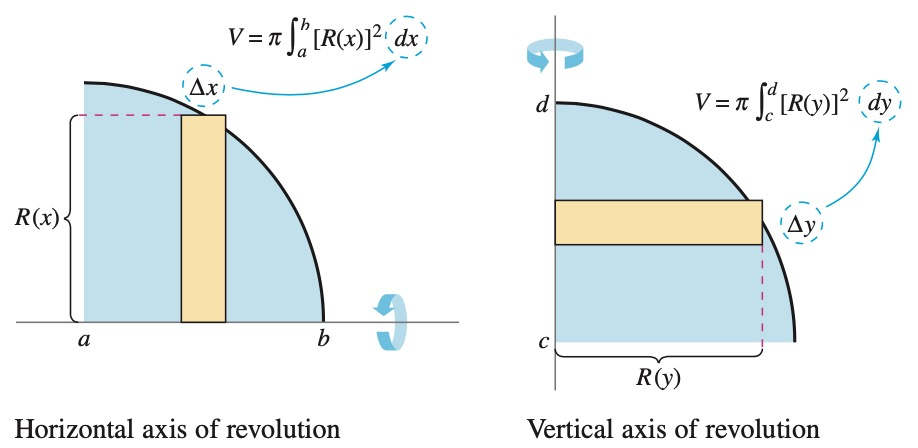
\includegraphics[width=1.0\linewidth]{Example_71.jpg} 
\end{minipage}

\begin{tcolorbox}[colback=examplebg, colframe=red!75!black, title=\textbf{EXAMPLE 1:  Using the Disk Method}, fonttitle=\bfseries, sharp corners]
Find the volume of the solid formed by revolving the region bounded by the graph of 
\[
f(x) = \sqrt{\sin x}
\]
and the $x$-axis ($0 \leq x \leq \pi$) about the $x$-axis.




\tcblower
\textbf{Solution:} 
From the representative rectangle in the upper graph, the radius of the solid is:
\[
R(x) = f(x) = \sqrt{\sin x}.
\]

Using the disk method, the volume of the solid of revolution is:
\[
V = \pi \int_a^b \big[R(x)\big]^2 \, dx.
\]

Substituting $R(x) = \sqrt{\sin x}$:
\[
V = \pi \int_0^\pi \big(\sqrt{\sin x}\big)^2 \, dx.
\]

Simplify:
\[
V = \pi \int_0^\pi \sin x \, dx.
\]

Integrate:
\[
V = \pi \big[-\cos x\big]_0^\pi.
\]

Evaluate:
\[
V = \pi \big[(-\cos \pi) - (-\cos 0)\big] = \pi \big[(-(-1)) - (-(1))\big] = \pi (1 + 1) = 2\pi.
\]

Thus, the volume of the solid is:
\[
V = 2\pi.
\]
\end{tcolorbox}


\begin{tcolorbox}[colback=examplebg, colframe=red!75!black, title=\textbf{EXAMPLE 2: Using the Disk Method}, fonttitle=\bfseries, sharp corners]

Revolve the region bounded by $y = x^3$, $y = 0$, and $x = 2$ around the $x$-axis. 
Setup the integral, but do not evaluate.

\tcblower
\textbf{Solution:} 
Using the Disk Method, the formula for the volume is:
\[
V = \pi \int_a^b \big[R(x)\big]^2 dx.
\]

Here, $R(x) = y = x^3$, and the bounds are $x = 0$ to $x = 2$. Thus, the integral setup is:
\[
V = \pi \int_0^2 (x^3)^2 dx = \pi \int_0^2 x^6 dx.
\]
\end{tcolorbox}


\begin{tcolorbox}[colback=examplebg, colframe=red!75!black, title=\textbf{EXAMPLE 3: Using the Disk Method}, fonttitle=\bfseries, sharp corners]

Revolve the region bounded by $y = 4 - x^2$, $y = 0$, and $x \geq 0$ around the $y$-axis. 
Setup the integral, but do not evaluate.

\tcblower
\textbf{Solution:} 
Using the Disk Method for rotation around the $y$-axis, the formula is:
\[
V = \pi \int_c^d \big[R(y)\big]^2 dy.
\]

Solve for $x$ in terms of $y$:
\[
y = 4 - x^2 \implies x^2 = 4 - y \implies x = \sqrt{4 - y}.
\]

Here, $R(y) = \sqrt{4 - y}$, and the bounds are $y = 0$ to $y = 4$. Thus, the integral setup is:
\[
V = \pi \int_0^4 (4 - y) dy.
\]
\end{tcolorbox}


\subsection{Volume with Disc
Method: Revolving
Around Other Axes}

\begin{mytheorem}{Volume with Disk Method for Revolving Around Other Axes}{}
    If a region is revolved around a horizontal line $y = c$ or a vertical line $x = c$, the volume of the resulting solid can be calculated using the Disk Method with adjusted radii. 

For a horizontal axis of revolution:
\[
V = \pi \int_a^b \big[R(x) - c\big]^2 dx,
\]
where $R(x)$ is the distance from the function to the axis of revolution.

For a vertical axis of revolution:
\[
V = \pi \int_c^d \big[R(y) - c\big]^2 dy,
\]
where $R(y)$ is the distance from the function to the axis of revolution
\end{mytheorem}


\begin{minipage}{\linewidth}
    \centering
    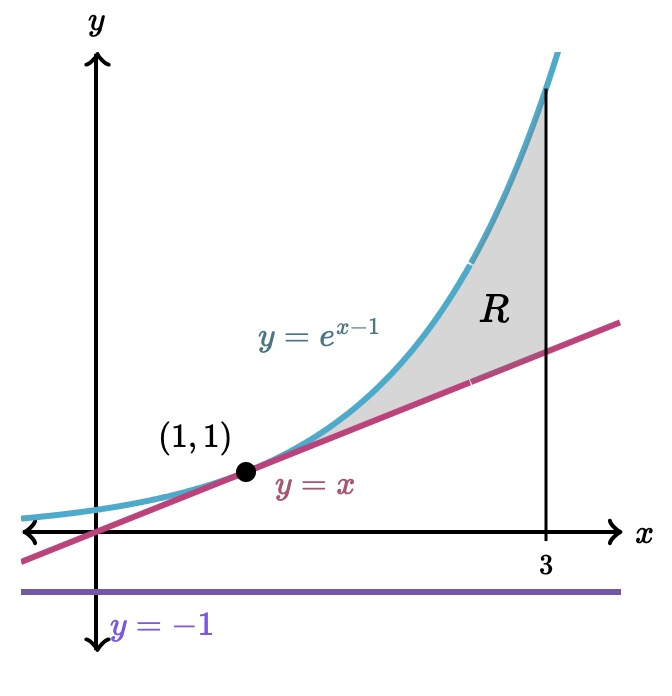
\includegraphics[width=0.55\linewidth]{Example_73.jpg} 
\end{minipage}


\begin{tcolorbox}[colback=examplebg, colframe=red!75!black, title=\textbf{EXAMPLE 1: Volume of Solid Generated by Rotating Region \( R \)}, fonttitle=\bfseries, sharp corners]

Given the region enclosed by:
\begin{itemize}
    \item \( y = 2 - x^2 \),
    \item \( y = 1 \),
\end{itemize}
revolve the region about the line \( y = 1 \). Find the volume of the resulting solid.

\tcblower
\textbf{Solution:} 
We use the disk method to find the volume.

\subsection*{Step 1: Determine the radius}
The radius is the vertical distance from \( y = 2 - x^2 \) to \( y = 1 \). This is given by:
\[
R(x) = (2 - x^2) - 1 = 1 - x^2.
\]

\subsection*{Step 2: Disk Method Formula}
The formula for the volume is:
\[
V = \pi \int_{-1}^{1} \big( R(x) \big)^2 \, dx.
\]

Substituting \( R(x) = 1 - x^2 \):
\[
V = \pi \int_{-1}^{1} \big( 1 - x^2 \big)^2 \, dx.
\]

\subsection*{Step 3: Expand the Integrand}
Expand \( \big( 1 - x^2 \big)^2 \):
\[
\big( 1 - x^2 \big)^2 = 1 - 2x^2 + x^4.
\]

So the volume becomes:
\[
V = \pi \int_{-1}^{1} \big( 1 - 2x^2 + x^4 \big) \, dx.
\]



\subsection*{Final Answer}
\[
V = \frac{16\pi}{15}.
\]



\end{tcolorbox}





\begin{tcolorbox}[colback=examplebg, colframe=red!75!black, title=\textbf{EXAMPLE 2: Volume of Solid Generated by Rotating Region \( R \)}, fonttitle=\bfseries, sharp corners]

Let \( R \) be the region enclosed by:
\begin{itemize}
    \item The line \( y = x \),
    \item The curve \( y = e^{x-1} \),
    \item The vertical line \( x = 3 \).
\end{itemize}

A solid is generated by rotating \( R \) about the line \( y = -1 \).

\textbf{Find:} The volume of the solid generated by the rotation.

\tcblower
\textbf{Solution:} 

The volume of the solid is calculated using the disk method. The radii of the disks are defined as follows:
\begin{itemize}
    \item Outer radius: \( R_{\text{outer}}(x) = e^{x-1} - (-1) = e^{x-1} + 1 \),
    \item Inner radius: \( R_{\text{inner}}(x) = x - (-1) = x + 1 \).
\end{itemize}

The volume is given by:
\[
V = \pi \int_{1}^{3} \Big[ \big( R_{\text{outer}}(x) \big)^2 - \big( R_{\text{inner}}(x) \big)^2 \Big] \, dx.
\]

Substitute the expressions for \( R_{\text{outer}}(x) \) and \( R_{\text{inner}}(x) \):
\[
V = \pi \int_{1}^{3} \Big[ \big( e^{x-1} + 1 \big)^2 - \big( x + 1 \big)^2 \Big] \, dx.
\]

Simplify:
\[
V = \pi \int_{1}^{3} \Big[ \big( e^{2(x-1)} + 2e^{x-1} + 1 \big) - \big( x^2 + 2x + 1 \big) \Big] \, dx.
\]

Finally, integrate:
\[
V = \pi \int_{1}^{3} \Big( e^{2(x-1)} + 2e^{x-1} - x^2 - 2x \Big) \, dx.
\]

Evaluate this integral to find the final volume.
\end{tcolorbox}



\subsection{Volume with Washer Method: Revolving Around the x- or y-Axis}

\begin{mytheorem}{Volume with Washer Method}{}
 To find the volume of a solid of revolution using the washer method, revolve a region about the horizontal (x-axis) or vertical (y-axis) axis. The volume is computed as follows:

\textbf{Revolution Around the x-Axis}
\[
V = \pi \int_{a}^{b} \Big( [R(x)]^2 - [r(x)]^2 \Big) \, dx,
\]
where:
\begin{itemize}
    \item \( R(x) \) is the outer radius,
    \item \( r(x) \) is the inner radius,
    \item \( a \) and \( b \) are the bounds of the region.
\end{itemize}

\textbf{Revolution Around the y-Axis}
\[
V = \pi \int_{c}^{d} \Big( [R(y)]^2 - [r(y)]^2 \Big) \, dy,
\]
where:
\begin{itemize}
    \item \( R(y) \) is the outer radius,
    \item \( r(y) \) is the inner radius,
    \item \( c \) and \( d \) are the bounds of the region.
\end{itemize}   
\end{mytheorem}

\begin{minipage}{\linewidth}
    \centering
    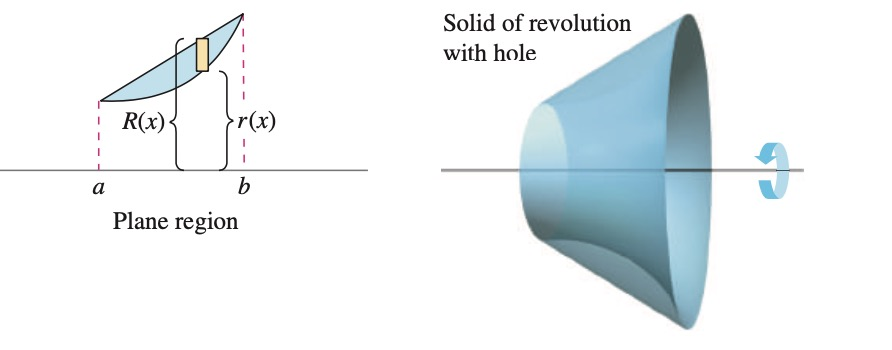
\includegraphics[width=1.0\linewidth]{Example_74.jpg} 
\end{minipage}


\begin{tcolorbox}[colback=examplebg, colframe=red!75!black, title=\textbf{EXAMPLE 1: Volume with Washer Method}, fonttitle=\bfseries, sharp corners]

Find the volume of the solid formed by revolving the region bounded by the graphs of 
\[
y = \sqrt{x} \quad \text{and} \quad y = x^2
\]
about the $x$-axis.



\tcblower
\textbf{Solution:} 

Find the volume of the solid formed by revolving the region bounded by the graphs of 
\[
y = \sqrt{x} \quad \text{and} \quad y = x^2
\]
about the $x$-axis.

\subsection*{Solution}
In Figure 7.20, you can see that the outer and inner radii are as follows:
\[
R(x) = \sqrt{x} \quad \text{(Outer radius)}, \quad r(x) = x^2 \quad \text{(Inner radius)}.
\]

Integrating between $0$ and $1$ produces:
\[
V = \pi \int_{a}^{b} \Big( [R(x)]^2 - [r(x)]^2 \Big) \, dx,
\]
\[
V = \pi \int_{0}^{1} \Big( (\sqrt{x})^2 - (x^2)^2 \Big) \, dx \quad \text{(Substitute $R(x)$ and $r(x)$)}.
\]

Simplify:
\[
V = \pi \int_{0}^{1} \Big( x - x^4 \Big) \, dx.
\]

Integrate:
\[
V = \pi \Bigg[ \frac{x^2}{2} - \frac{x^5}{5} \Bigg]_{0}^{1}.
\]


Final answer:
\[
V = \frac{3\pi}{10}.
\]


\end{tcolorbox}


\begin{tcolorbox}[colback=examplebg, colframe=red!75!black, title=\textbf{EXAMPLE 2: Volume with Washer Method(y-axis)}, fonttitle=\bfseries, sharp corners]

Find the volume of the solid formed by revolving the region bounded by the graphs of 
\[
y = x^2 + 1, \quad y = 0, \quad x = 0, \quad \text{and} \quad x = 1
\]
about the $y$-axis

\begin{minipage}{\linewidth}
    \centering
    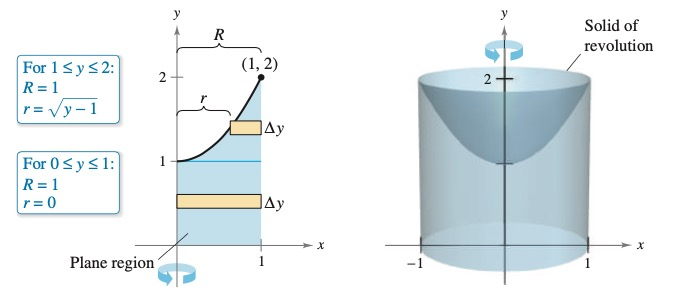
\includegraphics[width=0.80\linewidth]{Example_75.jpg} 
\end{minipage}
\tcblower
\textbf{Solution:} 
For the region shown in Figure, the outer radius is simply 
\[
R = 1.
\]

The inner radius is defined piecewise:
\[
r(y) = 
\begin{cases} 
0, & 0 \leq y \leq 1, \\
\sqrt{y - 1}, & 1 \leq y \leq 2.
\end{cases}
\]

Using this definition of the inner radius, you can use two integrals to find the volume:
\[
V = \pi \int_{0}^{1} \big(1^2 - 0^2\big) \, dy + \pi \int_{1}^{2} \big(1^2 - (\sqrt{y - 1})^2\big) \, dy.
\]

Simplify:
\[
V = \pi \int_{0}^{1} 1 \, dy + \pi \int_{1}^{2} \big(2 - y\big) \, dy.
\]

Integrate:
\[
V = \pi \Big[y\Big]_{0}^{1} + \pi \Big[2y - \frac{y^2}{2}\Big]_{1}^{2}.
\]

Evaluate:
\[
V = \pi (1 - 0) + \pi \Big[4 - 2 - 2 + \frac{1}{2}\Big].
\]


Final Answer:
\[
V = \frac{3\pi}{2}.
\]
\end{tcolorbox}




\subsection{Volume with Washer
Method: Revolving
Around Other Axes}
This section is about using the washer method plus revolving around other axes

\begin{mytheorem}{Revolving Around Other Axes}{}
 Revolving around other axes involves choosing a different vertical or horizontal line of either $x = a$ or $y = b$ to revolve around, instead of the $x$- or $y$-axis.

\textbf{General Equations}
For revolving around a horizontal line $y = b$, the volume is given by:
\[
V = \pi \int_{c}^{d} \big(f(x) - b\big)^2 \, dx.
\]

For revolving around a vertical line $x = a$, the volume is given by:
\[
V = \pi \int_{c}^{d} \big(f(y) - a\big)^2 \, dy.
\]

These formulas allow us to compute the volume of a solid of revolution when the axis of rotation is not one of the coordinate axes.   
\end{mytheorem}

The washer method removes the area of a circle of a small radius from the area of a circle with a bigger radius, creating a washer shape

\begin{mytheorem}{The Washer Method Around Other Axes}{}
    Using the principles of the washer method, when revolving around other axes, we use the following integral:

\[
V = \int_{c}^{d} \pi \big(f(x) - b\big)^2 - \pi \big(g(x) - b\big)^2 \, dx
\]

Here:
\begin{itemize}
    \item $f(x)$ represents the outer radius.
    \item $g(x)$ represents the inner radius.
    \item $b$ is the horizontal axis of revolution.
\end{itemize}

This formula accounts for the difference in radii, ensuring the volume of the hollow region is subtracted.
\end{mytheorem}


\begin{tcolorbox}[colback=examplebg, colframe=red!75!black, title=\textbf{EXAMPLE 1:  Washer Method Around Other Axes}, fonttitle=\bfseries, sharp corners]


Write the equation for the "big radius" and the "little radius" for the solid of revolution when revolving $S$ around the given line. Then set up the integral to find the volume of the solid formed. \textbf{Do not evaluate.}

\tcblower
\textbf{Solution:} 
\begin{enumerate}
    \item[a.] \textbf{The line $x = 3$:}
    \[
    R = 3, \quad r = 3 - y
    \]
    Volume:
    \[
    V = \pi \int_{0}^{3} \big[9 - (3 - y)^2\big] \, dy
    \]

    \item[b.] \textbf{The line $y = -1$:}
    \[
    R = 4, \quad r = x + 1
    \]
    Volume:
    \[
    V = \pi \int_{0}^{3} \big[16 - (x + 1)^2\big] \, dx
    \]

    \item[c.] \textbf{The line $x = -1$:}
    \[
    R = y + 1, \quad r = 1
    \]
    Volume:
    \[
    V = \pi \int_{0}^{3} \big[(y + 1)^2 - 1\big] \, dy
    \]
\end{enumerate}

\end{tcolorbox}


\end{document}








